\chapter{Placeholder for: A grounding in the domain}\label{chapter-preparing-the-ground}% 

\epigraph{`The Domain is the soul and record of all things Forerunner.'}{Halo: Silentium, pp 13-15, by Greg Bear}
% From https://www.halopedia.org/Domain, in turn from:
% Publisher ‏ : ‎ Gallery Books; Reprint edition (March 26, 2019)
% Language ‏ : ‎ English
% Paperback ‏ : ‎ 320 pages
% ISBN-10 ‏ : ‎ 198211181X
% ISBN-13 ‏ : ‎ 978-1982111816

\bigskip

\begin{kaobox}[frametitle=Context for this chapter]
\textbf{This chapter should only include material that provides context for these arguments:}\sidenote{Based on Arosha's framing for Chapter 1.}
\begin{enumerate}[start=3]
    \item Quality is particularly important for mobile app developers because of the way the ecosystem works.
    \item Software analytics can help improve quality, particularly with respect to reliability by gathering and analysing data relating to failures during real-world use.
    \item Analytics can be especially important for improving mobile app reliability because there is a huge diversity in devices and contexts where mobile apps are used, which can affect reliability of the apps.
\end{enumerate}
\end{kaobox}

% The following figure and subsequent paragraph is relocated from Chapter 3 (Related Work).
\begin{figure}[b!]
    \centering
    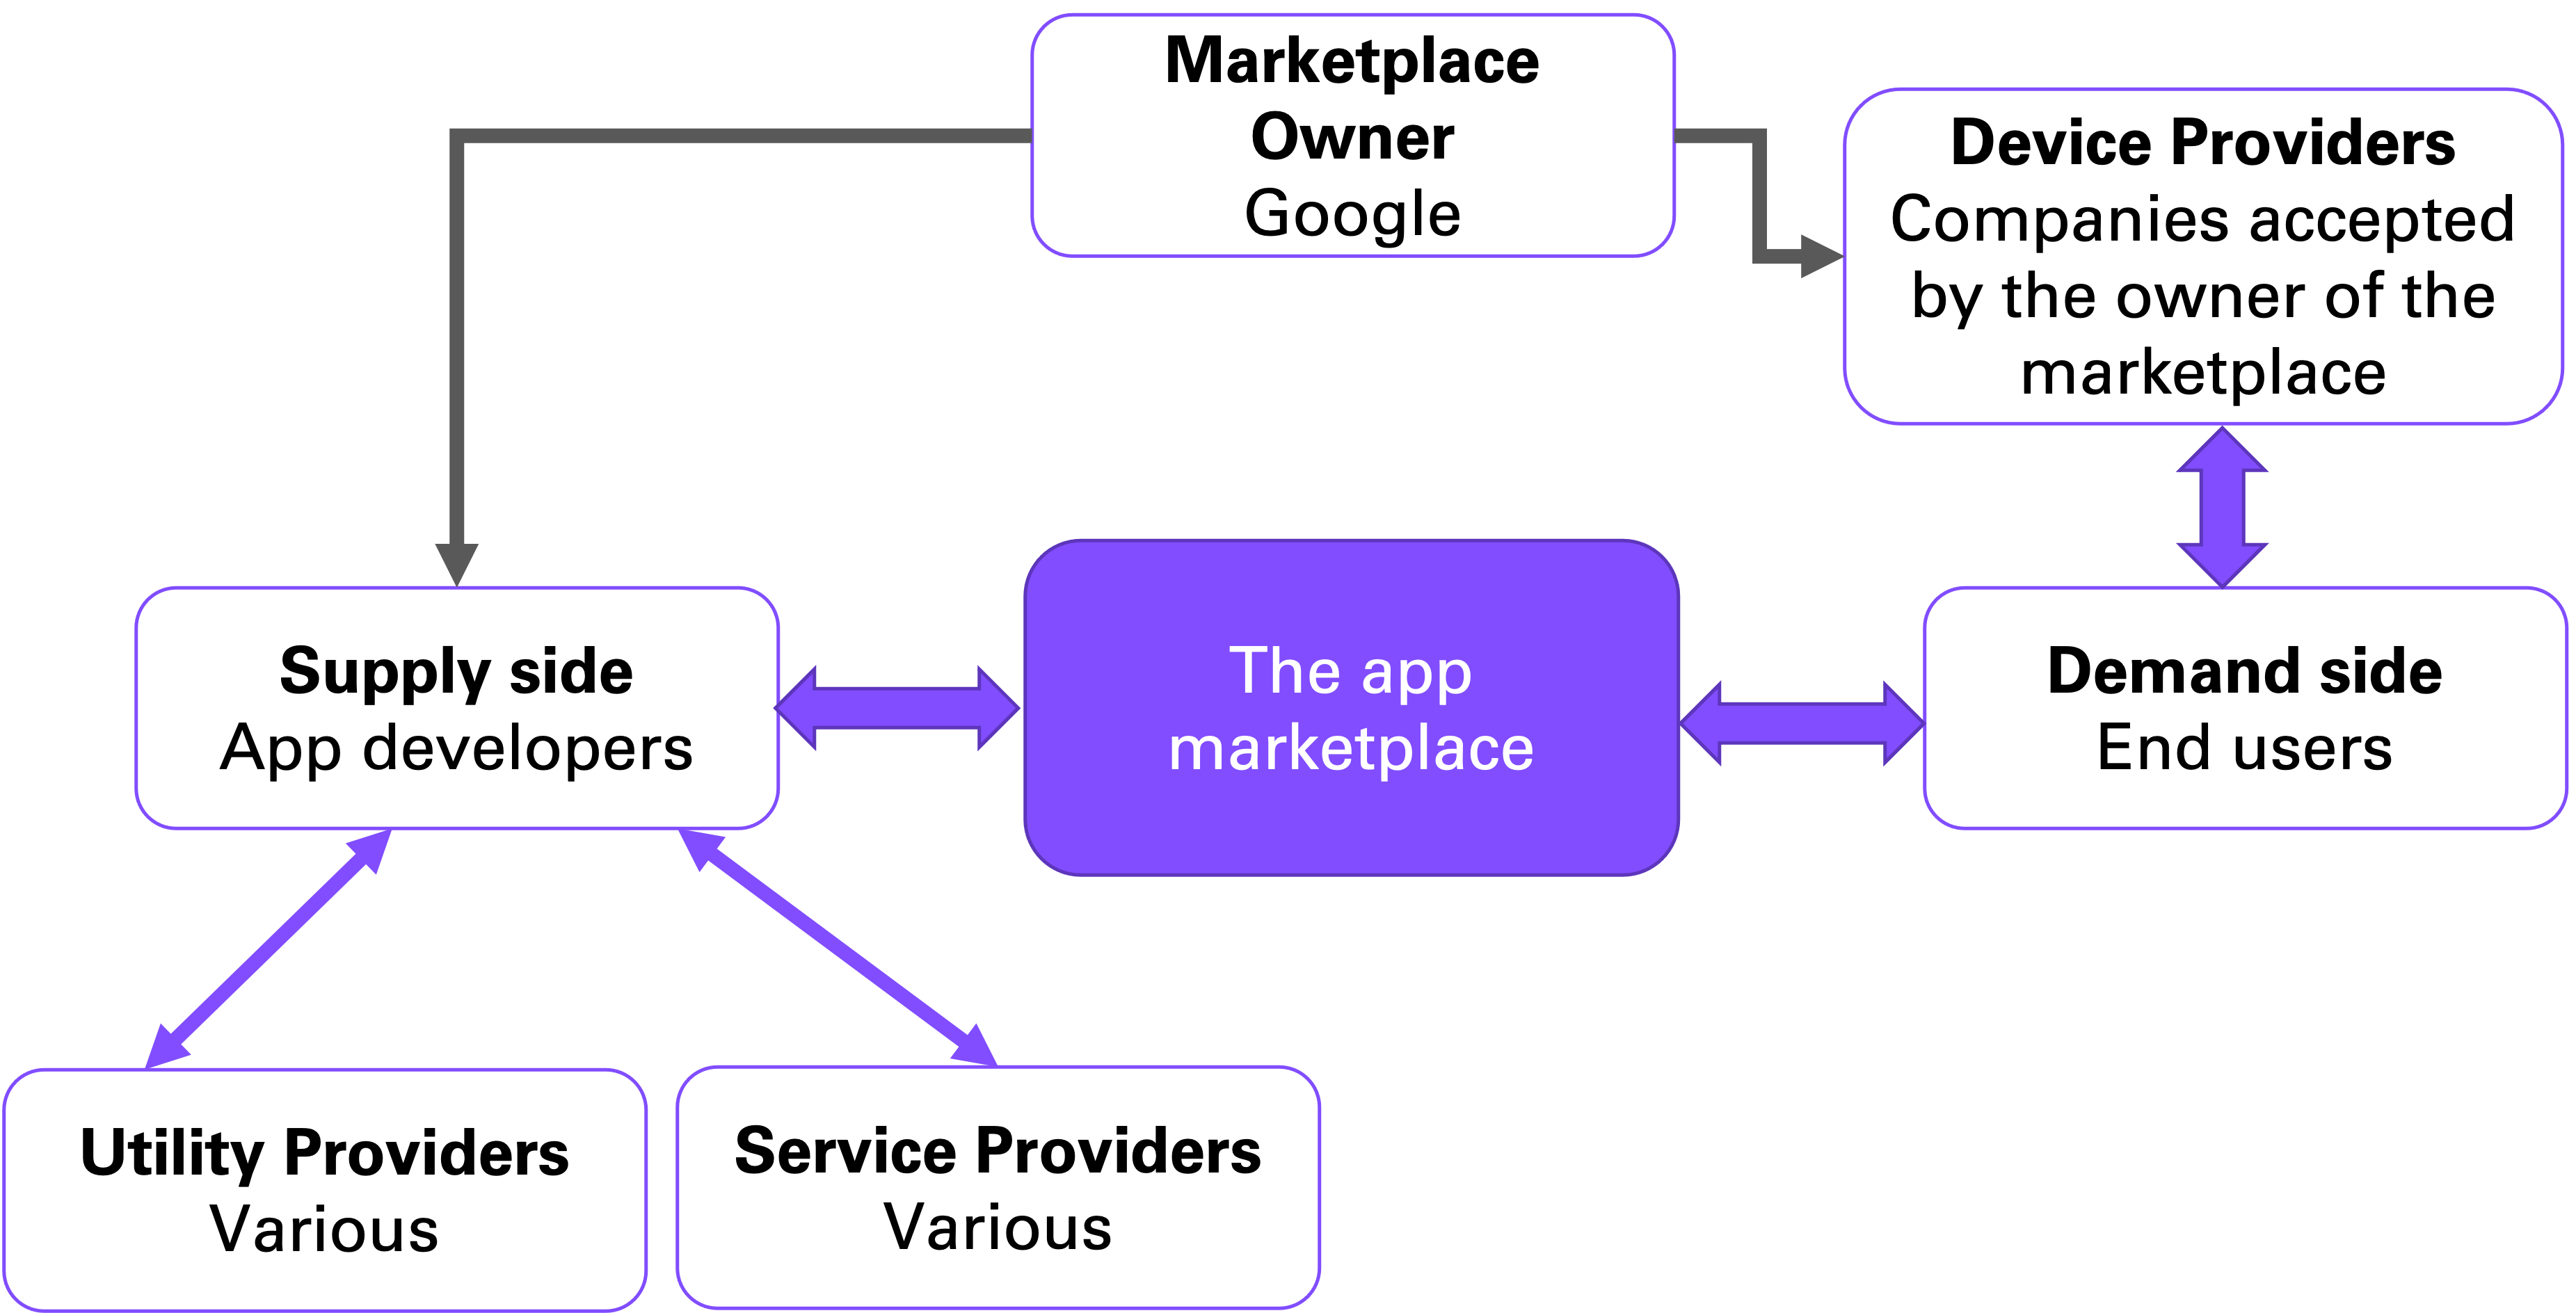
\includegraphics[width=0.9\linewidth]{images/my/android-app-ecosystem-main-players.png}
    \caption{The Modern Mobile App Ecosystem: Android}
    \label{fig:my_modern-mobile-app-ecosystem}
\end{figure}

As mentioned in the introduction, the mobile ecosystems touch on billions of people's lives, where flaws in the apps and the ecosystem can adversely affect the lives of many of those people. Figure~\ref{fig:my_modern-mobile-app-ecosystem} illustrates the main parties engaged in the ecosystem\sidenote{inspired by Figure 1, on p. 96 of \cite{KAPOOR2021_socio_technical_platform_ecosystems_etc}}, % TODO improve the formatting of the citation to add the authors, year, and title of the paper.
and it sets the context for the thesis and this chapter together with the research questions. The marketplace - the app store - establishes the ecosystem which generates revenues from the user population and frequently to a lesser extent from the makers -  the developers of the apps. Various providers of utilities and services offer these to the makers and they may also obtain revenues from one or more parties that are part of the ecosystem and/or from others, including advertisers. In the context of this research, utilities include software libraries such as the opensource logging service, Timber~\sidenote{\href{https://github.com/JakeWharton/timber}{github.com/JakeWharton/timber}}, where developers are responsible for any service provision. 
